\documentclass[a4paper,12pt]{article}
\usepackage{graphicx}
\begin{document}

\title{basic concepts}

The File Transfer Protocol (FTP) is a standard network protocol used to transfer computer files from one host to another host over a TCP-based network, such as the Internet.[1] FTP is built on a client-server architecture and uses separate control and data connections between the client and the server. FTP users may authenticate themselves using a clear-text sign-in protocol, normally in the form of a username and password, but can connect anonymously if the server is configured to allow it. For secure transmission that protects the username and password, and encrypts the content, FTP is often secured with SSL/TLS (FTPS). SSH File Transfer Protocol (SFTP) is sometimes also used instead, but is technologically different.

FTP may run in active or passive mode, which determines how the data connection is established.[2] In both cases, the client creates a TCP control connection from a random, usually an unprivileged, port N to the FTP server command port 21. In active mode, the client starts listening for incoming data connections from the server on port M. It sends the FTP command PORT M to inform the server on which port it is listening. By default, M=N. The server then initiates a data channel to the client from its port 20, the FTP server data port. In situations where the client is behind a firewall and unable to accept incoming TCP connections, passive mode may be used. In this mode, the client uses the control connection to send a PASV command to the server and then receives a server IP address and server port number from the server,[2][3] which the client then uses to open a data connection from an arbitrary client port to the server IP address and server port number received.[4] Both modes were updated in September 1998 to support IPv6. Further changes were introduced to the passive mode at that time, updating it to extended passive mode.[5]

The server responds over the control connection with three-digit status codes in ASCII with an optional text message. For example "200" (or "200 OK") means that the last command was successful. The numbers represent the code for the response and the optional text represents a human-readable explanation or request (e.g. <Need account for storing file>).[1] An ongoing transfer of file data over the data connection can be aborted using an interrupt message sent over the control connection.

\begin{figure}[ht!]
\centering
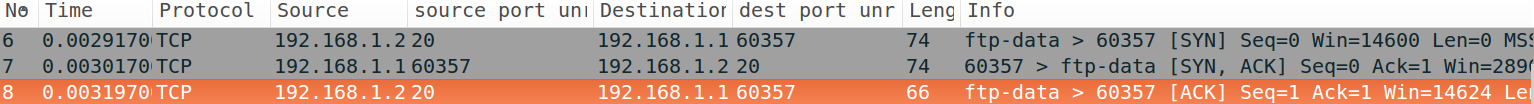
\includegraphics[width=90mm]{2.png}
\caption{A simple caption \label{overflow}}
\end{figure}

\reference
1.Forouzan, B.A. (2000). TCP/IP: Protocol Suite (1st ed.). New Delhi, India: Tata McGraw-Hill Publishing Company Limited.
2."Active FTP vs. Passive FTP, a Definitive Explanation". Slacksite.com. Archived from the original on 2014-12-31.
3.Parker, Don (September 2005). "Understanding the FTP Protocol". Windowsnetworking.com.
4.RFC 959 (Standard) File Transfer Protocol (FTP). Postel, J. & Reynolds, J. (October 1985).
5.RFC 2428 (Proposed Standard) Extensions for IPv6, NAT, and Extended Passive Mode. Allman, M. & Metz, C. & Ostermann, S. (September 1998).

\end{document}
